\makeheading{怎么办?地球上的沙子快要用完了\\Time  is  running out for sand}
\begin{multicols}{2}

你所住的大楼、喝水用的杯子和工作用的电脑有什么共同之处?答案是沙子. 这是现代生活中的关键原料,\qiangdiao{但意外的是,没有人知道现在还有多少沙子,又有多少正在被采挖}. 

What links the building you live in, the glass you drink from and the computer you work on? Sand. It is a key \emph{ingredient(因素)} of modern life and yet, surprisingly, no one knows how much sand there is or how much is being mined.

%\greyboxNID{\centering ingredient \textit{因素}}

\qiangdiao{沙子和砾石的采掘速度已经高于自然恢复的速度}. Mette Bendixen和他的同事们呼吁全球协力监管这项资源. 

\qiangdiao{Sand and \emph{gravel(沙砾)} are being  \emph{extracted(提取,采掘)} faster than they can be replaced. }Monitor and manage this resource globally, urge Mette Bendixen and colleagues.

%\greyboxNID{gravel 砂砾\hfill extract \textit{v.} extraction \textit{n.}提取,采掘}

\begin{figure}[H]
\centering
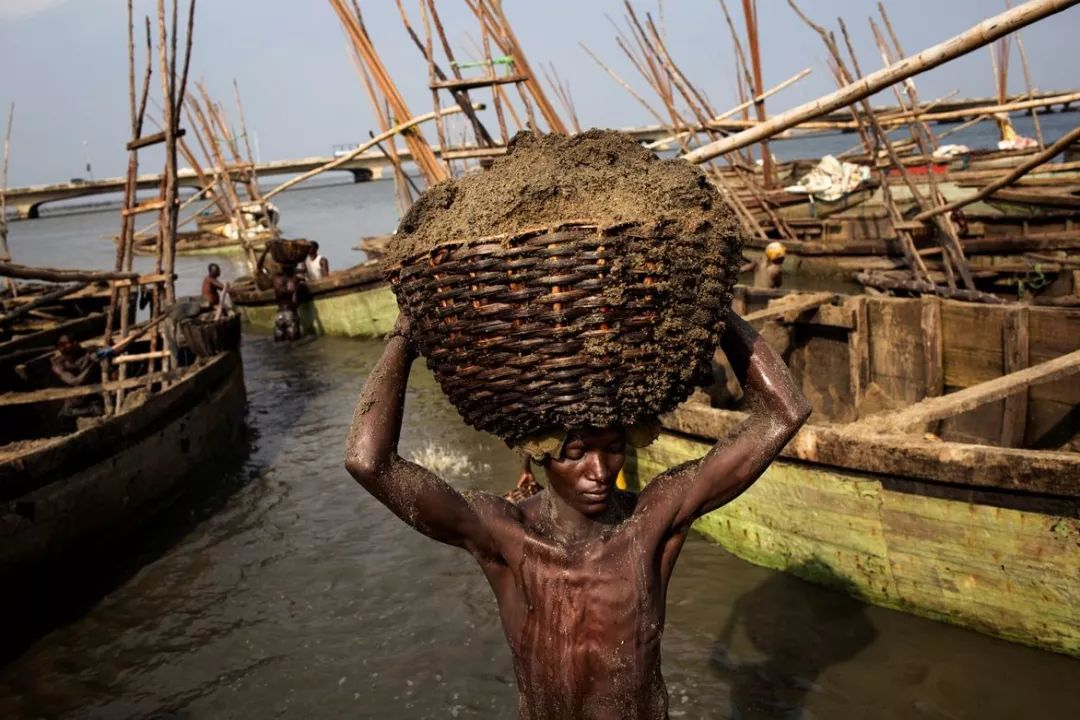
\includegraphics[width=\linewidth]{IMG/201911/image6.jpeg}
\caption{\textit{在尼日利亚的拉各斯潟湖里,沙工正在徒手从海床上挖沙. }}
\end{figure}




沙子和砾石是采掘量最大的一类原料,甚至超过了化石燃料. 需求大幅增加的原因是城市化和全球人口增长,尤其是中国、印度和非洲. 全世界每年大约会使用320-500亿吨沙子,主要用来制造水泥、玻璃和电子产品. 这个用量比自然再生率要高,因此到本世纪中叶,需求可能会超过供给,导致这种不可持续采挖的原因则是无知和忽视. 

Sand and gravel make up the most extracted group of materials, even exceeding fossil fuels.  \emph{Urbanization(城市化)} and global population growth are fueling an explosion in demand, especially in China, India and Africa. Roughly 32 billion to 50 billion tonnes are used globally each year, mainly for making concrete, glass and electronics. This exceeds the pace of natural renewal such that by mid-century, demand might exceed supply. A lack of knowledge and  \emph{oversight(疏忽)} is allowing this unsustainable  \emph{exploitation(开发)}.

%\greyboxNID{\centering oversight 疏忽\hfill exploit \textit{v.} exploitation \textit{n.} 开发\\urbanization 城市化}

\begin{figure}[H]
\centering
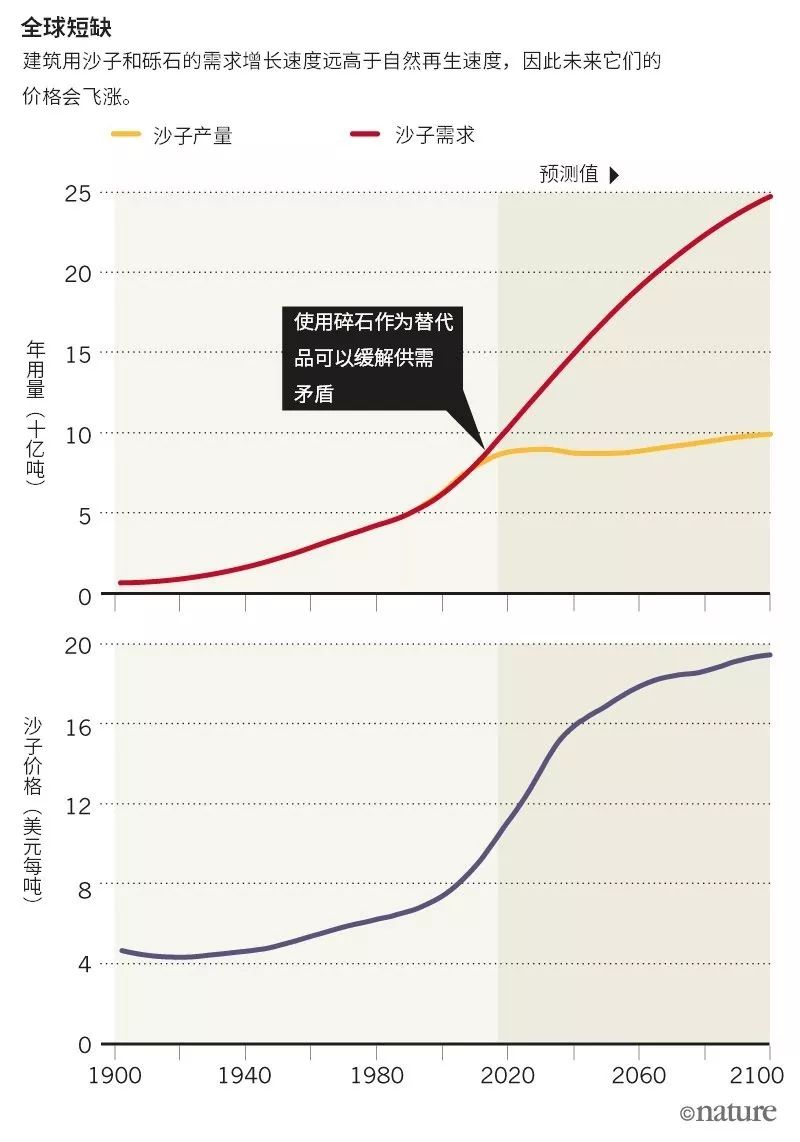
\includegraphics[width=\linewidth,clip=true,trim=0 40 0 120]{IMG/201911/image7.jpeg}
\vskip-2.5ex\mbox{}\hfill {\small ©nature}
\caption{\textit{建筑用沙子的需求增长速度远高于自然再生速度,因此它们的价格飞涨. }}
\end{figure}



\qiangdiao{沙漠里的沙子太过光滑,无法使用. 工业使用的有棱角的沙子绝大多数都来自于河流(占地球面积不到1\%). }在河里采挖沙子和砾石对生态环境、基础设施和沿河居住的30亿人口具有非常长远的影响. 例如,中国珠江因为采沙已经导致河床降低,使得抽取饮用水的难度加大,并损害了桥梁和河堤. 

\qiangdiao{Desert sand grains are too smooth to be useful, and most of the  \emph{angular(有尖角的)} sand that is suitable for industry comes from rivers (less than 1\% of the world’s land). }This extraction of sand and gravel has far-reaching impacts on ecology, infrastructure and the livelihoods of the 3 billion people who live along rivers. For example, sand mining on the Zhujiang in China has lowered water tables, made it harder to extract drinking water and damaged bridges and  \emph{embankments(堤岸)}.

%\greyboxNID{\centering angular 有尖角的\quad embankment 堤岸}

\begin{figure}[H]
\centering
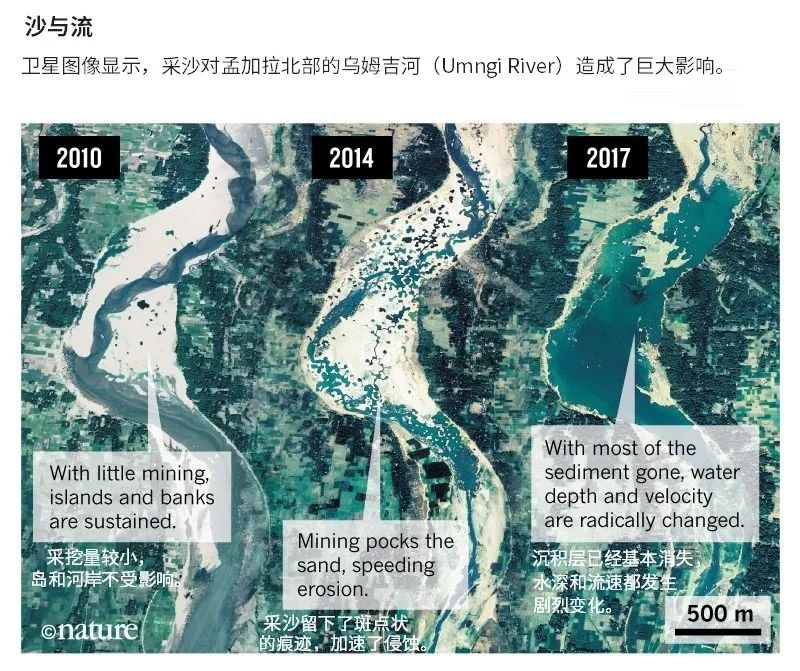
\includegraphics[width=\linewidth,clip=true,trim=20 0 20 130]{IMG/201911/image8.jpeg}
\vskip-2.5ex\mbox{}\hfill {\small ©Google Earth}
\caption{\textit{采沙对于孟加拉北部的乌姆吉河造成了巨大影响. }}
\end{figure}





大多数沙子贸易都未记录在案. 例如,2006年到2016年之间,新加坡报告从柬埔寨进口了8千万吨沙子,但柬埔寨确认出口的量只有不到4\%. \qiangdiao{大约70个国家或地区都存在猖獗的非法采沙行为. }过去十年来,包括印度和肯尼亚等国家有成百上千的人死于争沙冲突. 

Most of the trade in sand is undocumented. For example, between 2006 and 2016, less than 4\% of the 80 million tonnes of \emph{sediment(沉积物)} that Singapore reported having imported from Cambodia was confirmed as exported by the latter. \qiangdiao{Illegal sand mining is  \emph{rife(猖獗的)} in around 70 countries, }and hundreds of people have reportedly been killed in battles over sand in the past decade in countries including India and Kenya.

%\greyboxNID{\centering sediment 沉积物\quad rife 猖獗的}


所有这些问题在世界自然基金会(WWF)和联合国环境署(UNEP)的报告中都有所强调,报告也质疑采沙是否具有可持续性. \qiangdiao{问题的根源在于缺乏足够的数据和政策来引导人们以合理的速度消耗和采挖沙子. }

All these problems have been highlighted in reports from the wildlife charity WWF and the United Nations Environment Program (UNEP), questioning the sustainability of sand extraction. \qiangdiao{The  \emph{underlying(隐含的)} reasons are too few data and a lack of policies supporting responsible consumption and extraction}.

%\greyboxNID{underlie \textit{v.} 构成...的基础\hfill underlying \textit{adj.} 隐含的}

\section*{数据稀缺\quad Scant data}

当前对全球采沙量的估计并不可靠,无疑是过低了. 大多数关于河流沉积层的研究都在关注堤坝是如何阻拦水流的,学术界很少关注商业采沙. 此外,技术上,想要定量评估沙子如何移动或是沿河流如何沉积是很困难的. 

Current estimates of global sand mining are unreliable and undoubtedly too low. Most research on river sediment has focused on how dams block flows, and little academic attention has been given to  \emph{commercial(商业性的)} extraction. And it is technically hard to  \emph{quantify(定量分析)} how sand moves or is deposited along rivers.

%\greyboxNID{\centering scant 稀少的\quad commercial 商业性的\\quantify 定量分析}

在很多国家,采沙没有法律限制,可能会受当地的“采沙帮”控制. 采沙的方式从挖泥船加抽吸泵到空手铲都有,不分昼夜. 在需求最高的发展中国家,采沙大多是一种规模小且不规范的行业,因此很难监管和控制. 

In many countries, sand mining is unregulated and might involve local ‘sand  \emph{mafias(黑手党、小集团)}’. Methods of extraction range from dredging boats and suction pumping to digging with  \emph{shovels(铁铲)} and bare hands, both in daylight and during the night. In the developing world, where demand is greatest, it is mainly a small, informal industry, which is difficult to monitor and control.

%\greyboxNID{\centering mafia 本义为黑手党,这里引申为小集团 \\shovel 铁铲}

这对当地居民的生活和生物多样性造成了消极的影响. 例如,在湄公河三角洲,越南政府估计约有50万人需要从因采沙而塌陷的河岸搬离. 在印度北部的恒河,被侵蚀的河岸已经破坏了以鱼为食的恒河鳄的繁殖地. 这种濒危物种只剩下大约200只成年野生个体. 

This exerted a negative influence on the life of the locals and the bio-diversity. For example, in the Mekong delta, the Vietnamese government estimates that nearly 500,000 people will need to be moved away from river banks that are  \emph{collapsing(倒塌)} as a result of sand mining in the channel. In the Ganges River in northern India,  \emph{eroded(侵蚀)} river banks have destroyed the nesting and  \emph{breeding(繁殖)} habitats of fish-eating crocodiles, a critically endangered species with only around 200 adults left in the wild.

%\greyboxNID{\centering collapse 倒塌\quad erode 侵蚀\quad breed 繁殖}

\begin{figure}[H]
\centering
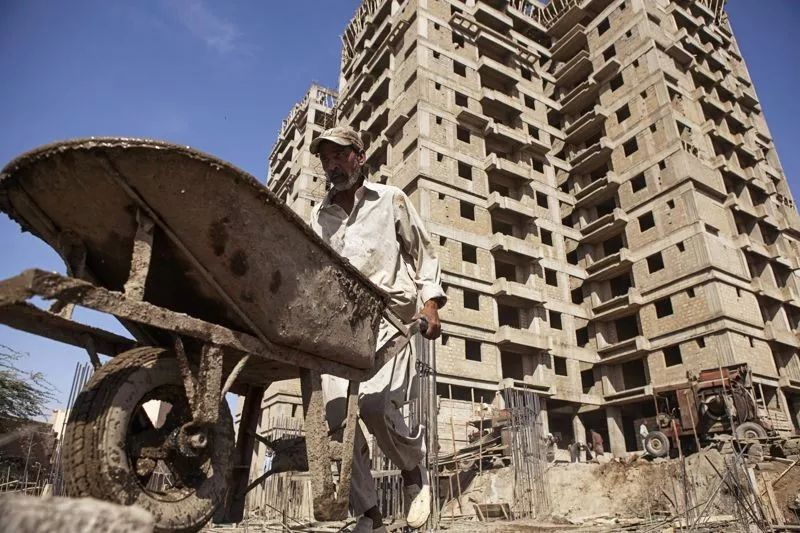
\includegraphics[width=\linewidth]{IMG/201911/image9.jpeg}
\caption{\textit{迅速的城市化和人口增长正在推升城市对建筑用沙的需求,例如巴基斯坦的卡拉奇市. }}
\end{figure}



\section*{全球议题\quad Global agenda}

以下七点对于采沙的可持续性至关重要. 

The following seven components are essential for sustainable sand extraction.

\qiangdiao{来源. }我们必须寻找并确证可持续性的沙子来源. 我们还要寻找不会影响河流的新被动沙源,采掘沉积在水坝后面的沙子;和下游的沙子相比,这对生态的影响可能会小一些. 

\qiangdiao{Source.} Sustainable sources of sand must be sought and certified. New passive sources of sand should be identified that do not damage rivers. Sand trapped behind dams might be extracted with less ecological  \emph{impact(深刻影响)} than mining downstream.

%\greyboxNID{\centering impact 深刻影响}


\qiangdiao{替代. }政府以及相关规划部门应当鼓励使用沙子的替代品,例如碎石、工业矿渣和废料,以及回收塑料. 例如,公路、停车场和车道可以将塑料垃圾包裹在沥青中,以减少沙子的用量. 


\qiangdiao{Replace.} Governments and planning  \emph{authorities(权力,当局)} should encourage greater use of alternatives to sand, such as crushed rock, industrial slag and waste and recycled plastic. For example, roads, car parks and driveways made from plastic waste  \emph{embedded(并入,嵌入)} in  \emph{asphalt(沥青)} can lessen demand of sands.

%\greyboxNID{\centering embed 并入, 嵌入\quad authority 权力, 当局\quad asphalt 沥青}

\qiangdiao{再利用. }沙基材料应当尽可能地回收利用. 例如,拆迁时产生的废物和混凝土可以压碎后重新混合到水泥中. 

\qiangdiao{Reuse.} Sand-based materials should be reused when possible. For example, demolition waste and concrete can be crushed and mixed into cement. 



\qiangdiao{减少需求. }减少新建筑物中的混凝土需求量同样可以减少对沙子的需求. 这可以通过使用更高效的材料(\textit{例如空心的混凝土块})实现. 

\qiangdiao{Reduce.} Cutting the amount of concrete required in new structures would also lessen the demand for sand. This could be achieved by using more efficient materials (\textit{such as \emph{hollow}(中空的) concrete blocks}). 

%\greyboxNID{\centering hollow 中空的}

\qiangdiao{治理. }首先,UNEP和WTO应当制定全球性的采沙指南. 此外,应当建立起国际或多边的政策框架,来规范并控制沙子的采挖. 

\qiangdiao{Govern.} UNEP and the WTO should establish global good-practice guidelines for sand extraction as a first step. An international framework to regulate and control sand extraction should be \emph{forged(确立)}. 

%\greyboxNID{\centering forge 确立}


\qiangdiao{教育. }政府、科学家和工业界必须宣传有关采沙问题的信息,从学校到政策建议再到媒体并且必须同时宣传问题的解决方式. 

\qiangdiao{Educate.} Governments, scientists and industry must spread information on the issues of sand mining,  from schools to policy advice and media coverage, and must be covered along with solutions to the problems.


\qiangdiao{监测. }一个全球性的数据收集和分享项目至关重要,它可以定量统计采沙的地点和规模,以及全球河沙的自然波动. 另外重力回溯及气候实验卫星可以揭示河口的沉积物流量,以及排入海中的成分. 

\qiangdiao{Monitor.} A global program to gather and share data is important for quantifying the location and extent of sediment mining, as well as the natural variations in sand \emph{flux(变动)} in the world’s rivers. Furthermore, satellite data from the Gravity Recovery and Climate Experiment (GRACE) can reveal sediment \emph{discharge(排放)} rates at river outlets and material exported to the ocean.

%\greyboxNID{\centering flux 变动\quad discharge 排放}

NASA的“地表水与海洋地形”(\textit{Surface Water and Ocean Topography})任务预计于2021年发射. 它将监测宽度超过100米的大河的流量,其覆盖规模是前所未有的. 

NASA’s Surface Water and Ocean Topography mission, due to launch in 2021, will offer \emph{unprecedented(前所未有的)} coverage of water discharge in large rivers more than 100 meters wide. 

%\greyboxNID{\centering unprecedented 前所未有的}

我们还需要可以在地面上验证这些数据的工具,包括测量站、用来测量河床形态和沉积物流量的声学技术、以及空中激光雷达. 现在,很多船只都会携带声纳或回声测深仪,它们可以产生大量关于河流和河口的地形数据. 

Tools to confirm such findings on the ground will be needed, including \emph{gauge(测量)} stations, \emph{acoustic(声学的)} technologies for measuring river-bed morphology and sediment fluxes, and airborne lidar. Many boats now \emph{routinely(常规的)} carry sonar or echo sounders, which offer a huge resource of \emph{topographic(地形的)} data about the world’s rivers and \emph{estuaries(河口)}. 

%\greyboxNID{\centering routinely 常规的\quad gauge 测量\quad estuary 河口

%acoustic 声学的\quad topographic 地形的}

UNEP和WWF的报告已经在沙子里踏下了一个重重的脚印. 现在,法规和我们的行动必须跟上. 

The UNEP and WWF reports are important footprints in the sand. Now they must be followed up with regulation and our actions.

\end{multicols}\vskip-5em
\makeheading{课内知识拓展·右手螺旋定则}
\begin{multicols}{2}

在静磁、电磁感应的探索过程中,我们学习了三种“手法”:右手螺旋定则、左手定则、右手定则. 往往在一个问题的处理过程中,左手和右手剑拔弩张,几乎快打成了个“中国结”. 有没有统一的方法在电磁学的海洋中辨别方向呢?

答案是肯定的. 

首先我们先引入一种新的矢量运算——叉乘,规

\noindent\begin{minipage}[t]{0.6\linewidth}
定:矢量$\vec{a}$叉乘$\vec{b}$的大小为:$|\vec{a}\times\vec{b}|=|\vec{a}||\vec{b}|\sin \theta$. 与此同时,矢量的叉乘结果仍为矢量,它具有方向,可用右图所示的右手螺旋定则判断. 
\end{minipage}
\begin{minipage}[t]{0.4\linewidth}\vskip-1em
\begin{figure}[H]
    \centering
    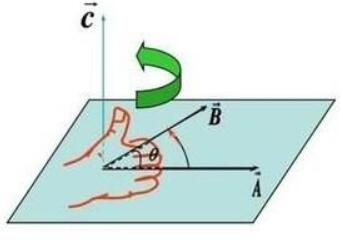
\includegraphics[width=\linewidth]{IMG/201911/image4.jpeg}
\end{figure}
\end{minipage}

此时再看前所学的洛伦兹力的方向,$F=q\vec{v}\times\vec{B}$:右手四指指向速度方向,弯曲转向磁场方向并握住,此时大拇指即为受力方向,注意若为负电荷,应反向. 

应注意的是,$\vec{a}\times\vec{b}$与$\vec{b}\times\vec{a}$的结果不同,即矢量叉乘不满足交换律,应用右手螺旋定则可发现,$\vec{a}\times\vec{b}$与$\vec{b}\times\vec{a}$正好反向. 因此公式中适量的前后顺序不要记反. 

学会了吗?可以试着把安培力$F=I\vec{L}\times\vec{B}$($\vec{L}$\textit{的方向为电流流向}),地转偏向力(\textit{科里奥利}力)$F=-2m\vec{\omega}\times\vec{v}$($\vec{\omega}$\textit{的方向由南极指向北极})表示出来噢. 
\end{multicols}
\vskip-3em
\ADxinhangdao

\vfill
\noindent\rule{\linewidth}{0.5pt}
\noindent\begin{minipage}[b]{0.69\linewidth}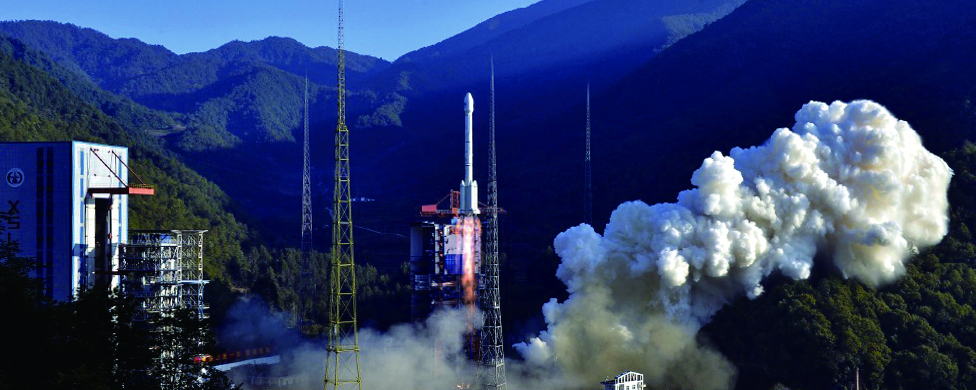
\includegraphics[width=\linewidth]{IMG/201911/005SySbsly1g97w7lpy7nj33sw2j4e82.jpg}\end{minipage}\hfill
\begin{minipage}[b]{0.29\linewidth}
\subsection*{北斗导航网络又添新成员}
\emph{  \emph{11}月\emph{23}日\emph{8}时\emph{55}分,我国在西昌卫星发射中心用长征三号乙运载火箭及配套远征一号上面级,以“一箭双星”方式成功发射第五十、五十一颗北斗导航卫星. 卫星顺利进入预定轨道. 本次是长征系列运载火箭的第\emph{319}次飞行. \hfill 南勇\emph{/}摄}
\end{minipage}\vskip-0.25cm
\noindent\rule{\linewidth}{0.5pt}

\ADhairui\newpage
\makeheading{生活中的科学·上期答案}
\begin{multicols}{2}
\noindent\qiangdiao{Q1 电脑黑色的壁纸会比白色的壁纸省电吗?}

这个结论要根据电脑屏幕类型具体分析. 

现在大家使用的电脑显示器绝大多数都是液晶显示器. 液晶显示器本身并不会发光,而是分为两个部分:液晶面板和背光模块. 只要不关闭屏幕,背光模块始终在发光,而开关掌握在液晶模块手里. 液晶模块中的液晶分子仅允许特定方向振动的光通过,有光到达前面板的像素点,在人看来就是亮的. 
\begin{figure}[H]
\centering
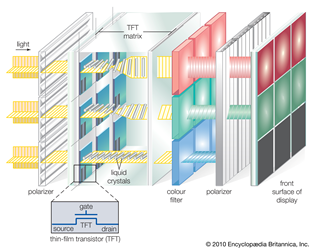
\includegraphics[width=0.7\linewidth]{IMG/201911/image1.png}
\end{figure}

主流的液晶显示屏技术分为TN,IPS 和 VA,区分的方式很简单. 一般来说 TN 屏可视角度较差,不是正对着屏幕的话,看到的屏幕颜色会失真. 而 VA 屏和 IPS 可视角度会大很多,屏幕看起来更加均匀. 对于 TN 屏来说,液晶分子在不加电压的情况下呈现螺旋状,正好允许光通过,此时屏幕上对应的像素点是亮的. 而在晶体管施加电压后,液晶分子变成同一取向,此时对应屏幕上的像素点是暗的. 所以如果你的电脑屏幕是 TN 屏,黑色的壁纸会比白色的壁纸稍微费一点电. 而 VA 屏和 IPS 屏幕正好相反,液晶分子默认不通电的情况下不让背光通过,屏幕是暗的,所以使用黑色的壁纸则会稍微省一点电. 

PS:其实比起颜色,将屏幕的亮度调低,使用时间就能显著延长哦. 

\noindent\qiangdiao{Q2 超市里的扶梯是怎样卡住购物车的?}

逛超市的时候,购物车为什么能够卡在手扶梯上呢?到了下扶梯的时候又能够很自然的脱落呢?

细心的同学一定会发现,手扶梯的梯面上布满了一道道凹槽,而在将购物车推到电梯上时会观察到购物车的轮子陷在凹槽中,感觉被卡住了. 事实上也的确如此,如下图所示,车轮由橡胶制的外圆、内圆以及刹车块构成,外圆的轮胎宽度与电梯表面的凹槽宽度接近,当购物车被推上电梯时,车轮外圆嵌入电梯表面的凹槽,轮胎侧面和凹槽侧面间的摩檫力使得车轮无法向前运动;刹车块的作用是为了防止出现车轮外圆磨损严重导致摩擦力减小或者无法侧面形成摩檫力时,轮胎整个陷入凹槽仍然可以行驶的情况,在车轮外圆接触凹槽底部时,刹车块与梯面接触,提供摩擦力,使得购物车无法移动. 

\begin{figure}[H]
\centering
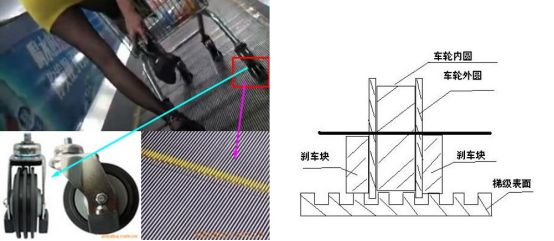
\includegraphics[width=\linewidth]{IMG/201911/image2.jpeg}
\end{figure}

在购物车行驶到电梯尽头,由于自动扶梯表面和电梯出口处的挡板一般成一定夹角,同时也具有凹槽状条纹,可以使嵌入电梯凹槽的车轮逐渐抬升,脱离凹槽,恢复正常行驶. 

\noindent\qiangdiao{Q3 为什么粥和牛奶在冷却时会在表面形成一层膜?}

我们从粥和牛奶的成分分析,米粥主要成分是淀粉,而牛奶主要是水、蛋白质、脂肪、乳糖等. 

牛奶中的脂肪不溶于水,蛋白质将脂肪包裹,形成乳浊液. 饮用的牛奶经特殊处理后使脂肪球变得相对较小,这样覆盖在脂肪球表面的蛋白质膜的张力就不会很大,牛奶长期存放也不会分层. 而一但加热,原本较为稳定的脂肪球结构瓦解,脂肪和蛋白质会散开、上浮. 蛋白质相互交联在一起形成膜,脂肪吸附在蛋白质膜上,这就是我们所说的奶皮. 

而粥皮的主要成分是淀粉,烧粥的时候,淀粉受热吸水糊化,而冷却的时候,表面水分散失,导致淀粉链间距变小,形成网状的淀粉膜,这就是我们所说的粥皮. 这个过程和纸张的干、湿同样都是大分子和水之间的作用产生的结果,在一定程度上相似. 

\noindent\qiangdiao{Q4 为什么用手刮小票会有黑色纹路?}

生活中常用的小票一般都是热敏打印纸. 其制造原理是就是在原有的纸张上涂一层热敏变色层,一种在受热条件下会出现显色反应的染料. 和我们常用的喷墨打印机相比,这个“墨”一开始就在纸上,只是要受热才显色. 这样就清楚了,当手指甲快速划过,产生的热量就会在小票上留下黑色纹路了!

\end{multicols}


\newpage
\makeheading{双十一没“剁手”到底亏不亏?}
\begin{multicols}{2}

\noindent
\includegraphics[width=0.5\linewidth]{IMG/201911/image10.png}
\hfill
\begin{minipage}[b]{0.48\linewidth}
\rule{2em}{0em}刚刚过去的“双十一”,想必一定有同学享受了一夜之间剁手清空购物车的快感,也有同学为自己忙于学习无暇参与购物狂欢而感到遗憾. 每年双十一,不论折扣规则
\end{minipage}

\noindent 有多复杂,优惠力度多模糊,都挡不住全民疯狂购物的冲动. 

虽然这些剁手的理由看起来都很正常,但是这些贪图优惠购买的商品又有多少是你真正需要的呢?根据一位国内学者的统计研究,\qiangdiao{消费者对于这些冲动性消费商品的不满比例高达62\%. 没错,双十一当天购买的商品很可能不是你真正需要的. }

双十一之前,无数人彻夜不眠研究淘宝复杂的促销规则,不断对比哪些商品买得划算,想要在双十一占到便宜. 他们的心理可能是这样的:毕竟现在不买,以后恢复原价再购买,那岂不是血亏!

为什么我们会觉得没有占到便宜就是血亏呢?这都要归因于“损失厌恶”心理,由经济学家卡尼曼提出. \qiangdiao{他认为人们失去一件事物时的痛苦程度,要比得到这件事物所感受到的幸福程度更大. }

我们可以试着做一个抛硬币的小游戏. 如果硬币朝上,你将会得到100元,如果硬币朝下,你将会损失50元,你会选择玩这个小游戏吗?

分析这个游戏,硬币朝上和朝下的概率都是50\%,赢了得到100元,输了损失50元. 从数学期望上来分析,我们应该参与这个游戏. 

如果你的答案是不参与,那么恭喜你落入多数人的群体. 人们损失厌恶的心理,使得对于损失的敏感度要远高于对得到的敏感度. 卡尼曼的进一步研究还证实了\qiangdiao{人们损失一件事物的痛苦程度,大约是得到这件事物的幸福程度的两倍. }



“双十一不买就是血亏”印证了这个心理学原理. \qiangdiao{其实人们在乎的并不是优惠本身,而是有没有占到这个便宜. }想到恢复原价后再购买就会产生\qiangdiao{心理上的损失感,为了避免损失厌恶带来的不愉快,}人们纷纷将双十一成交额合力推上新台阶. 

众多商家也在精明地反向利用损失厌恶,想方设法减少人们在付款的时候产生的“痛苦程度”. 试想一下,如果在购买价格高昂的商品时,商家均要求全额支付,恐怕销售额将会大幅下降. 于是各大电商平台纷纷推出了分期付款的功能,将大额消费拆分成小额还款,从而大大减少了付款时候的“痛苦”,消费者“剁手”的冲动也就更难遏制了. 

\qiangdiao{尽管“双十一打折还不买就是吃亏”的心理很正常,但因此导致的购物行为却不一定是理性的. }

\end{multicols}
\vskip-3em
\noindent\greybox{\vskip-25pt
\makeheading{生活中的科学}

\qiangdiao{Q1 使用电脑或手机时应该充着电用还是快没电时再充电呢?}

\rule{3ex}{0em}(Tips: 电池类型为锂离子电池 )

\qiangdiao{Q2 为什么黑笔的笔芯后有一团黄色液体?}

\rule{3ex}{0em}(Tips:注意在使用笔芯过程中黄色液体的位置)

\qiangdiao{Q3 为什么锯齿边可以帮助我们更容易撕开包装呢?}

\rule{3ex}{0em}(Tips: 从受力角度考虑)

\qiangdiao{Q4 水杯接水时,离出水口近和离出水口远哪种方式接水速度更快?}

\rule{3ex}{0em}(Tips: 可利用基本运动学公式计算)
}\hskip0.5em
\ADyixuehui